\documentclass[11pt]{article}

% load some asm stuff -
\usepackage{amssymb}
\usepackage{amsmath}
\usepackage{amsthm}
%\usepackage{palatino,lettrine}
\usepackage{fancyhdr}
\usepackage{epsfig}
\usepackage[square,sort,comma,numbers]{natbib}
\usepackage{simplemargins}
\usepackage{setspace}
\usepackage{wrapfig}
%\usepackage{boiboites}
\usepackage[margin=0pt,font=small,labelfont=bf]{caption}
\usepackage{framed}
\usepackage{lipsum}


\bibliographystyle{plos2009}

% Set the size
%\textwidth = 6.75 in
%\textheight = 9.75 in
%\oddsidemargin = 0.0 in
%\evensidemargin = 0.0 in
%\topmargin = 0.01 in
%\headheight = 0.0 in
%\headsep = 0.25 in
%\parskip = 0.15in
\doublespace

\setallmargins{1in}

\newtheorem{example}{Example}[section]
\newtheorem{thm}{Theorem}[section]
\newtheorem{property}{Property}[section]

\theoremstyle{definition}
\newtheorem{defn}[thm]{Definition}

\makeatletter
\renewcommand\subsection{\@startsection
	{subsection}{2}{0mm}
	{-0.05in}
	{0.5\baselineskip}
	{\normalfont\normalsize\bfseries}}
\renewcommand\subsubsection{\@startsection
	{subsubsection}{2}{0mm}
	{-0.05in}
	{-0.5\baselineskip}
	{\normalfont\normalsize\bfseries}}
\renewcommand\paragraph{\@startsection
	{paragraph}{2}{0mm}
	{-0.05in}
	{-0.5\baselineskip}
	{\normalfont\normalsize\itshape}}
\makeatother
\linespread{1.2}

\fancypagestyle{proposal}{\fancyhf{}%
	\fancyhead[RO,LE]{\thepage}%
	\fancyhead[LO,RE]{CHEME 3130 Chemical Engineering Thermodynamics}%
	\renewcommand\headrulewidth{1pt}}
\pagestyle{proposal}

% Box -
%\usepackage{framed,color}
\usepackage{mdframed}
\definecolor{lgray}{rgb}{0.92,0.92,0.92}
\definecolor{lsalmon}{rgb}{1.0,0.63,0.48}

% Single space'd bib -
\setlength\bibsep{0pt}

\renewcommand{\rmdefault}{phv}\renewcommand{\sfdefault}{phv}
%\newboxedtheorem[boxcolor=black, background=gray!5,titlebackground=orange!20,titleboxcolor = black]{color_box_example}{Example}{test}

% Change the number format in the ref list -
\renewcommand{\bibnumfmt}[1]{#1.}

% Change Figure to Fig.
\renewcommand{\figurename}{Fig.}

%Joycelyn Chan, Joshua Lequieu, Michael Paull, Chidanand Balaji, Ryan Tasseff
%Our derivation follows closely the earlier development of Fredrickson \citep{Fredrickson:1976fk}.

% Begin ...
\begin{document}

%\begin{titlepage}
{\par\centering\textbf{\Large CHEME 3130: Equations of state for pure substances}}
\vspace{0.2in}
{\par \centering \large{Jeffrey D. Varner$^{*}$}}
\vspace{0.05in}
{\par \centering \large{$^{*}$}Robert Frederick Smith School of Chemical and Biomolecular Engineering}
{\par \centering \large{Cornell University, Ithaca NY 14853}}
\vspace{0.1in}
{\par \centering \small{Copyright \copyright\ Jeffrey Varner 2017. All Rights Reserved.}}\\

%\end{titlepage}
\date{}
\thispagestyle{empty}

\setcounter{page}{1}

\begin{mdframed}[backgroundcolor=lgray]
\subsection*{Previously:}
\noindent We introduced the energy balance for an open and closed system.
An open system allows both mass and energy transfer between the system and its surroundings:
\begin{eqnarray*}\label{eqn:general-open-balance}
	\frac{d}{dt}\Bigl[m\left(u+\frac{1}{2}\bar{v}_{s}^{2}+gz\right)\Bigr]_{sys} &=& \dot{Q}+\dot{W}_{sh}+
	\sum_{s=1}^{\mathcal{S}}\nu_{s}\left(h_{s}+gz_{s}+\frac{1}{2}\bar{v}_{s}^{2}\right)\dot{m}_{s}+
	\sum_{r=1}^{\mathcal{R}}\dot{e}_{r}\\\label{eqn:total-mass-balance}
	\frac{dm}{dt} &=& \sum_{s=1}^{\mathcal{S}}\nu_{s}\dot{m}_{s}
\end{eqnarray*}
While no mass transfer is allowed between the system and the surroundings for a closed system.
We derived the differential forms for the closed energy balances (closed first law):
\begin{eqnarray*}
	\delta{Q} &=& C_{V}dT+\left[\left(\frac{\partial U}{\partial V}\right)_{T}+P\right]dV\\
	\delta{Q} &=& C_{P}dT+\left[\left(\frac{\partial U}{\partial P}\right)_{T}+P\left(\frac{\partial V}{\partial P}\right)_{T}\right]dP
\end{eqnarray*}where $C_{P}$ and $C_{V}$ denote the constant pressure and constant volume heat capacities, respectively.
Mechanical work in a closed system was given by $\delta{W}=-P_{e}dV$, where $P_{e}$ denotes the external pressure (of the surroundings).
The external pressure $P_{e}\simeq P$ (external pressure equals the system pressure) for reversible expansion or contraction operations.

\subsection*{Student outcomes:}
At the end of this lecture module, you will be able to:
\begin{itemize}
  \item[O$_1$]{Describe the assumptions associated with, and the similarities and differences between the ideal gas law, cubic equations of state, and the Virial equation of state}
  \item[O$_2$]{Use the ideal and cubic equations of state to calculate the reversible work for isothermal and adiabatic expansion/contraction of gases}
  \item[O$_3$]{Describe pressure-temperature (PT) and pressure-volume (PV) phase diagrams, the triple and critical points.}
\end{itemize}
\end{mdframed}

\clearpage

% * [](<#phase-behavior>)
% * [The Virial equation of state](<#virial-eos>)
% * [Cubic equations of state and van der Waals equation](<#cubic-eos>)
% * [Data driven equations of state](<#data-driven-eos>)

\subsection*{Introduction}
Equations of state are mathematical models of the behavior of pure materials, or mixture of materials as a function of physical conditions and composition.
Equations of state are critically important because the physical knobs that we can adjust for chemical engineering processes
are the temperature $T$, pressure $P$ and volume $V$ of the system.
However, these three properties are not independent;
we typically write a single property, for example the volume of system, as a function of the temperature $T$ and the pressure $P$, which
are independent parameters that can be adjusted for some technological benefit. Thus, we rely on an equation of state to \emph{predict} properties e.g., the volume
from the independent parameters.

\begin{wrapfigure}{l}{0.55\textwidth}\center
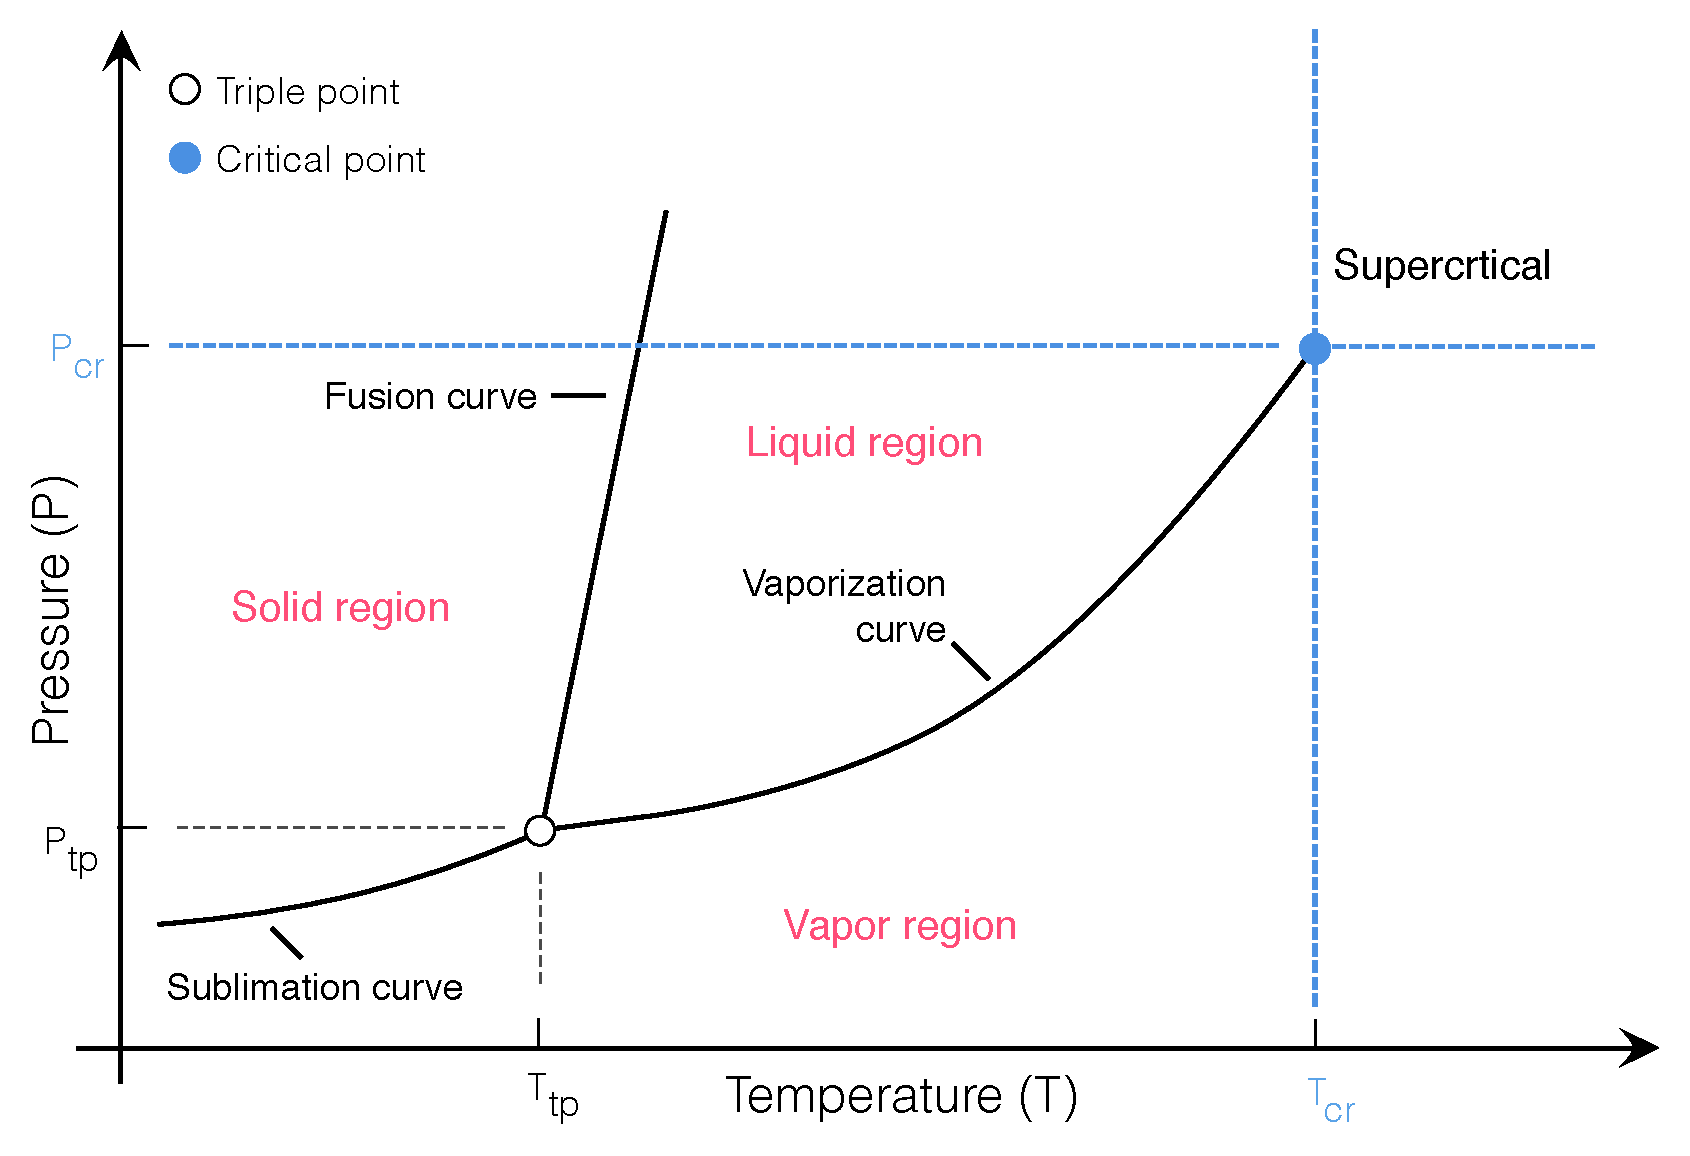
\includegraphics[width=0.54\textwidth]{./figs/PT-Diagram.pdf}
\caption{Hypothetical pressure temperature (PT) phase diagram for a pure material.}\label{fig-phase-diagrams}
\end{wrapfigure}

Consider a typical pressure temperature (PT) phase diagram for a pure substance (Fig. \ref{fig-phase-diagrams}, top).
As we move around the (P,T) space, pure substances assume different physical forms (phases) ranging from a solid, liquid or gas to a fourth regime,
the supercritical phase which has fluid like properties.
The solid lines on the PT-diagram are borders which demarcate phase transitions e.g., changing from a solid to a gas (sublimation curve)
or a liquid to a gas (vaporization curve).
At (P,T) points far away from these transitions, substances exists as a pure phase e.g., a liquid or gas only;
however, directly on these curves both phases exist in a mixture.
At a special point called the triple point (P$_{\mathrm{tp}}$,T$_{\mathrm{tp}}$) all three phases coexist.
Continuing up the vaporization curve, we arrive at the critical point (P$_{\mathrm{cr}}$,T$_{\mathrm{cr}}$).
When temperature and pressure exceed the critical values, the differences between liquid and gas phases disappear,
leading to a homogeneous supercritical fluid.
Supercritical fluids have many industrial applications \cite{SupercriticalFluids}.


\subsection*{Equation of state models}
An equation of state is a function $\mathcal{F}(\cdot)$ that described how the state variables, temperature $T$, pressure $P$, volume $V$ and composition $n$
of a system are related, such that:
\begin{equation}
\mathcal{F}\left(P,T,V,n\right) = 0
\end{equation}
Thus, equations of state are mathematical models of the physical behavior of pure substances, or mixtures with a few modifications.
The structure of an equation of state can be motivated by our understanding of the physics of the molecules in a system, or can also be data driven mathematical constructs.
Ultimately, the origin of an equation of state is irrelevant; given that their primary purpose is the prediction of system properties, if predictions are good it does not
matter how we arrived at the particular functional form for an equation of state. Let's discuss are few common equations of state that you likely use in process
calculations.

\subsubsection*{Ideal Gas Law (IGL).}~One of the simplest equations of state is the ideal gas law (IGL):
\begin{equation}
  Pv-RT = 0
\end{equation}
The IGL ignores both the volume of the molecules in the gas, and all interactions between them (hard-sphere model)
other than collisions with the wall of the container and each other.
The attractiveness of the ideal gas law comes from our ability to derive it from first principles;
the functional form for the ideal gas law can be derived from the kinetic theory of gases (discussed in almost every physical chemistry textbook).
However, the IGL does not accurately describe gas phase behavior at realistic pressures, not does it describe phase transitions.
Despite this, the IGL is often used for \textit{quick~and~dirty} process calculations, even though it is technically valid in only in the
limit of zero pressure.

% The most significant advancements of the vdW equation was its description of molecular interactions;
% its parameters describe the volume occupied by fluid particles (excluded volume),
% and the interactions between particles (both features ignored by the ideal gas law).
% In particular, the van der Waals parameters $a$ and $b$ are associated with the van der Waal force,
% and the size of the molecules in the fluid (excluded volume), respectively.

\subsubsection*{Cubic Equations of State.}
Cubic equations of state were developed to address the limitations of the ideal gas law.
The general form for this class of equation of state is given by:
\begin{equation}
v^{3}+f_{1}(T,P)v^2+f_{2}(T,P)v+f_{3}(T,P) = 0
\end{equation}
where $f_{j}(T,P)$ are specific functions of temperature $T$ and pressure $P$ for each instance of cubic state equation.
Arguably, the best known cubic equation of state is van der Waals (vdW) equation:
\begin{equation}
  \displaystyle P = \frac{RT}{v-b} - \frac{a}{v^2}
\end{equation}
\begin{figure}\center
  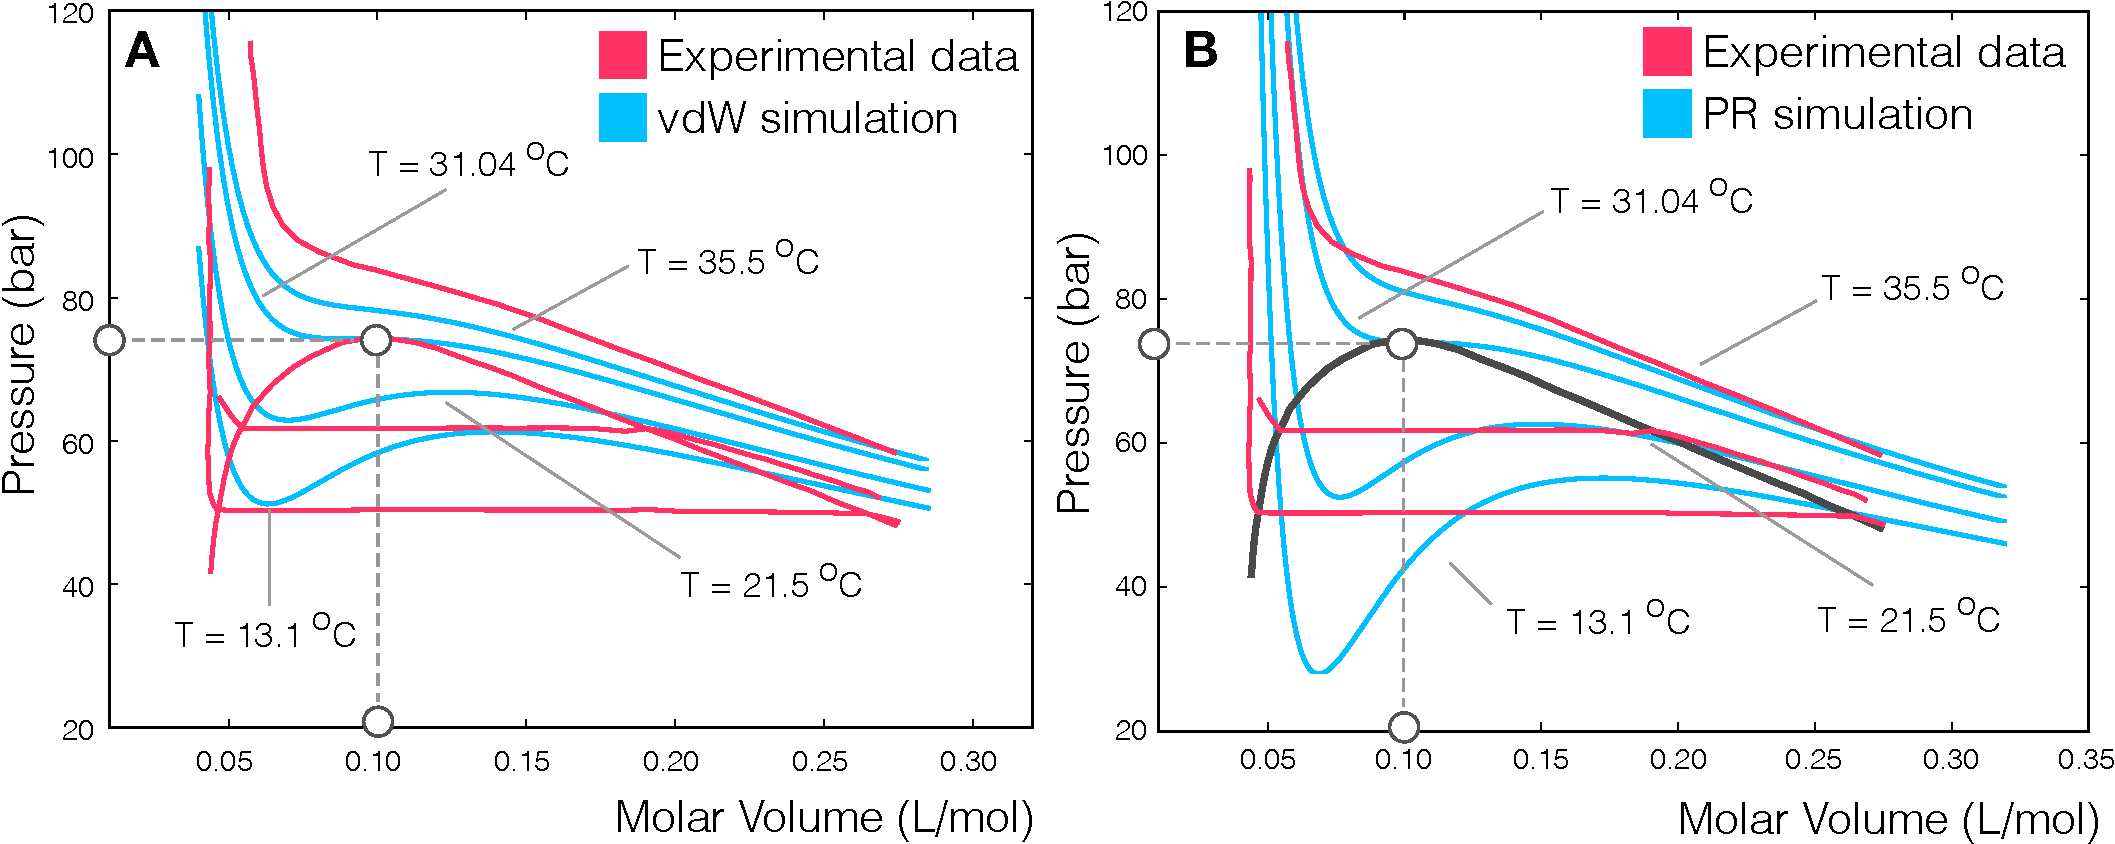
\includegraphics[width=1.0\textwidth]{./figs/Fig-CubicEOS.pdf}
  \caption{Pressure volume behavior of CO$_{\mathrm{2}}$.
	A: vdW equation prediction of the PV behavior of CO$_{\mathrm{2}}$ for different temperatures versus data.
	B: Peng-Robinson equation prediction of the PV behavior of CO$_{\mathrm{2}}$ for different temperatures versus data.}  \label{fig-cubic-eos}
\end{figure}

The vdW equation of state was proposed by the Dutch physicist Johannes Diderik van der Waals in his Ph.D thesis published in 1873 at the University of Leiden
\cite{vdW-Thesis}; he later won the Nobel prize for this work in 1910.
The first term in the vdW equation is the volume-corrected ideal gas law;
the parameter $b$ describes the volume occupied by the molecules of the gas. Thus $v-b$ describes the molar volume that is not occupied by the gas moleculues.
The second term in the vdW equation describes the attraction between molecules; this term describes how potential energy interactions between molecules influences the pressure
and is parameterized by the vdW parameter $a$.
The vdW parameters can be estimated directly from data (as van der Waals himself did), potentially from first-principles statistical mechanical calculations,
or from analytical expressions derived based upon the behavior of the fluid near the critical point.

\begin{mdframed}[backgroundcolor=lgray]
\noindent\textbf{Example}.~Estimate van der Waals parameters from critical point data.
At the critical point P=P$_{\mathrm{cr}}$, T=T$_{\mathrm{cr}}$ and v=v$_{\mathrm{cr}}$;
all three roots of the vdW equation must equal v$_{\mathrm{cr}}$:
\begin{equation}
  \left(v-v_{\mathrm{cr}}\right)^3 = 0
\end{equation}
After we expand the term in parenthesis we get:
\begin{equation}
v^3-\left(3v_{\mathrm{cr}}\right)v^2+\left(3v^{2}_{\mathrm{cr}}\right)v-v^{3}_{\mathrm{cr}} = 0
\end{equation}
The vdW equation in standard form is given by:
\begin{equation}
  v^3-\left(b+\frac{RT_{\mathrm{cr}}}{P_{\mathrm{cr}}}\right)v^2+\frac{a}{P_{\mathrm{cr}}}v-\frac{ab}{P_{\mathrm{cr}}} = 0
\end{equation}
Term by term comparison of the powers of the molar volume gives three equations:
\begin{equation}
  3v_{\mathrm{cr}} = b+\frac{RT_{\mathrm{cr}}}{P_{\mathrm{cr}}}\qquad
  3v^{2}_{\mathrm{cr}} = \frac{a}{P_{\mathrm{cr}}}\qquad
  v^{3}_{\mathrm{cr}} = \frac{ab}{P_{\mathrm{cr}}}
\end{equation}
Solving these three equations for v$_{\mathrm{cr}}$, $a$ and $b$ in terms of P$_{\mathrm{cr}}$ and T$_{\mathrm{cr}}$ gives:
\begin{equation}
  v_{\mathrm{cr}} = \frac{3}{8}\frac{RT_{\mathrm{cr}}}{P_{\mathrm{\mathrm{cr}}}}\qquad
  a = \frac{27}{64}\frac{R^{2}T^{2}_{\mathrm{cr}}}{P_{\mathrm{cr}}}\qquad
  b = \frac{1}{8}\frac{RT_{\mathrm{cr}}}{P_{\mathrm{cr}}}
\end{equation}
Although these estimates for $v_{\mathrm{cr}}$, $a$ and $b$ may not be optimal, they can be estimated from
tabulated critical values that are often available (in contrast to PVT data which is not as abundant).
\end{mdframed}

% ##### Exercises
% * [Show that van der Waals equation is a cubic equation of state](./VDL-CubicEqnOfState.md)
% * [Estimate the parameters in the van der Waals equation of state](./VDL-Parameters.md)

\subsection*{Modifications to vdW equation of state}
vdW was considered one of the most significant contributions to Thermodynamics since Boyle's work in the 17th century (Boyle's law, published in 1662, see \cite{West:2005aa}).
However, it does not correctly predict gas-liquid behavior for most applications.
Towards this issue, there have been many modifications to the vdW equation to correct its performance \cite{Valderrama2003}.
These modifications can all be generated from the generic cubic equation of state model:
\begin{equation}\label{eq:generic-model}
P = \frac{RT}{\left(v-b\right)}-\frac{a(T)}{\left(v+\epsilon b\right)\left(v+\sigma b\right)}
\end{equation}
For a given equation of state, $\epsilon$ and $\sigma$ are constants (the same for all substances), while
$a(T)$ and $b$ are substance specific. The temperature dependence model, $a(T)$, is specific to each equation of state.
Similar to vdW, we can derive analytical expressions for the $a(T)$ and $b$ in terms the critical temperature and pressure:
\begin{equation}
	a\left(T\right) = \Psi\left[\frac{\alpha\left(T_{r}\right)R^{2}T^{2}_{\mathrm{cr}}}{P_{\mathrm{cr}}}\right]\qquad
	b = \Omega\left[\frac{RT_{\mathrm{cr}}}{P_{\mathrm{cr}}}\right]
\end{equation}

\begin{center}
\begin{tabular}{lccccc}
	\hline\\
	Eq. of State & $\alpha\left(T_{r}\right)$ & $\sigma$ & $\epsilon$ & $\Omega$ & $\Psi$ \\\\
	\hline\\

	vdW (1873) & 1 & 0 & 0 & 1/8 & 27/64 \\
	RK (1949) & T$_{r}^{-1/2}$ & 1 & 0 & 0.08664 & 0.42748 \\
	SRK (1972) & $\alpha_{SRK}\left(T_{r},\omega\right)$ & 1 & 0 & 0.08664 & 0.42748 \\
	PR (1976) & $\alpha_{PR}\left(T_{r},\omega\right)$ & 1+$\sqrt{2}$ & 1 - $\sqrt{2}$ & 0.07779 & 0.45724 \\\\

	\hline

\end{tabular}
\end{center}


One way to correct the IGL for higher pressures, is to use a correction in the form of a Virial equation of state.
Suppose we define a dimensionless constant $Z$, called the compressibility factor, as $Z \equiv {Pv}/{RT}$.
A Virial equation of state is the power-series in either pressure $P$ or
inverse powers of the molar (or specific) volume $v$:
\begin{equation}
  \displaystyle Z \equiv \frac{Pv}{RT} = \sum_{i=0}^{\infty}\alpha_{i}v^{-i}\qquad
  \displaystyle Z \equiv \frac{Pv}{RT} = \sum_{i=0}^{\infty}\alpha^{\prime}_{i}P^{i}
\end{equation}
where $\alpha_{i},\alpha^{\prime}_{i}$ denotes Virial coefficients.
The Virial coefficients $\alpha_{i}$ and $\alpha^{\prime}_{i}$ (which are related with one another)
describe the strength of intermolecular interactions (interactions between molecules) in the fluid.
These coefficients can be estimated from data for each material of interest, or can be derived
from first-principle statistical mechanical calculations given a potential function which describes the strength of interactions between molecules.
The Virial coefficients are given by:
\begin{eqnarray*}\nonumber
	\alpha_{0}=\alpha^{\prime}_{0} &=& 1 \\
	\alpha_{1}^{\prime} &=& \frac{\alpha_{1}}{RT}\\\nonumber
  \alpha_{2}^{\prime} &=& \frac{\alpha_{2}-\alpha_{1}^2}{\left(RT\right)^2}\\\nonumber
  & \vdots &
\end{eqnarray*}

\clearpage

\begin{mdframed}[backgroundcolor=lgray]
  \noindent\textbf{Example}: Estimate the second Virial coefficient $\alpha_{1}$ as a function of temperature from CH$_{\mathrm{4}}$ compressibility data.

	\vspace{0.2in}

	\noindent\textbf{Solution}:
	Keeping up to first order term, the compressibility factor as a function of pressure gives:
	\begin{equation}\label{eq:first-order-Z}
		Z = 1 + \alpha^{\prime}_{1}P
	\end{equation}We can estimate $\alpha^{\prime}_{1}$ from the derivative of the power series expansion.
	The coefficient $\alpha^{\prime}_{1}$ is the slope of the compressibility versus pressure;
	differentiating the Z pressure power series with respect to pressure gives:
	\begin{equation}
		\frac{dZ}{dP} = \sum_{i=0}^{\infty}i\cdot\alpha^{\prime}_{i}P^{i-1}
	\end{equation}from which:
	\begin{equation}
		\frac{dZ}{dP} = \alpha^{\prime}_{1} = \frac{\alpha_{1}}{RT}
	\end{equation}when $i~=~1$. Substituting the expression for $\alpha^{\prime}_{1}$ in terms of $\alpha_{1}$ into Eqn. \eqref{eq:first-order-Z} gives:
	\begin{equation}
		Z = 1 + \left(\alpha_{1}/RT\right)P
	\end{equation}
\end{mdframed}

\clearpage



\subsubsection*{Data driven equations of state}
Suppose we know the molar (or specific) volume of a pure substance (in either the liquid, gas or solid phase) at some temperature $T_{o}$ and pressure $P_{o}$, denoted by $v_{o}(T_{o},P_{o})$.
Instead of developing a model for how the molar or specific volume changes as we move around the entire $PT$-space (which is complicated by phase transitions), lets develop an expression for $v(T,P)$ in the neighborhood of $(T_{o},P_{o})$ by a Taylor expansion of $v(T,P)$:
\begin{equation}
  \displaystyle dv \simeq \left(\frac{\partial v}{\partial T}\right)\Bigr|_{P}dT + \left(\frac{\partial v}{\partial P}\right)\Bigr|_{T}dP
\end{equation}
Dividing both sides of the Taylor approximation by the molar (or specific volume) and then integrating:
\begin{equation}
  \displaystyle \int_{v_{o}}^{v}\frac{dv}{v} = \int_{T_{o}}^{T} \frac{1}{v}\left(\frac{\partial v}{\partial T}\right)\Bigr|_{P}dT+\int_{P_{o}}^{P}\frac{1}{v}\left(\frac{\partial v}{\partial P}\right)\Bigr|_{T}dP
\end{equation}
gives (after some algebraic rearrangement):
\begin{equation}
\displaystyle v \simeq v_{o}\exp\left(\beta\Delta{T}-\kappa\Delta{P}\right)
\end{equation}
where $\beta\equiv\frac{1}{v}\left(\frac{\partial v}{\partial T}\right)\Bigr|_{P}$ and $\kappa = -\frac{1}{v}\left(\frac{\partial v}{\partial P}\right)\Bigr|_{T}$ are referred to as the volume expansivity and the isothermal compressibility,
respectively and $\Delta{P}=P-P_{o}$ and $\Delta{T}=T-T_{o}$.

\clearpage

\begin{mdframed}[backgroundcolor=lgray]
  \noindent\textbf{Example}: For liquid acetone at 20$^{\mathrm{o}}$C and 1 bar:
  \begin{equation*}
    \beta = 1.5\times10^{-3}~^{\mathrm{o}}\mathrm{C}^{\mathrm{-1}}\qquad\kappa=62\times10^{-6}~\mathrm{bar}^{-1}\qquad v~=~1.3~\mathrm{ml~g^{-1}}
  \end{equation*}
  For acetone estimate:
  \begin{enumerate}
    \item[(a)]{The value of $\Bigr(\partial{P}/\partial{T}\Bigr)_{v}$}
    \item[(b)]{The pressure generated by heating at constant volume from 20$^{\mathrm{o}}$C and 1 bar to 30$^{\mathrm{o}}$C}
    \item[(c)]{The change in volume for a change from 20$^{\mathrm{o}}$C and 1 bar to 0$^{\mathrm{o}}$C and 10 bar}
  \end{enumerate}
	\noindent\textbf{Solution}
	\begin{enumerate}
		\item[(a)]{The approximate equation of state reduces to:
		\begin{equation}
			\beta dT -\kappa dP = 0
		\end{equation}
		at constant volume. Rearranging the constant volume equation of state gives:
		\begin{equation}
			\left(\frac{dP}{dT}\right)_{v} = \frac{\beta}{\kappa} = 24~\mathrm{bar~^{o}C^{-1}}
		\end{equation}
		}
		\item[(b)]{Lets assume that $\beta$ and $\kappa$ are constant across the 10$^{\mathrm{o}}$C temperature difference.
		At constant volume, we can solve for dP:
		\begin{equation}
			dP = \left(\frac{\beta}{\kappa}\right)dT
		\end{equation}Integrating the pressure expression:
		\begin{equation}
			\int_{P_{0}}^{P_{1}}dP = \int_{T_{0}}^{T_{1}}\left(\frac{\beta}{\kappa}\right)dT
		\end{equation}gives:
		\begin{equation}
			P_{1} = P_{0}+\left(\frac{\beta}{\kappa}\right)\Delta{T}
		\end{equation}Substituting in the values for $\Delta{T}$, $\beta$ and $\kappa$ gives:
		\begin{equation}
			P_{1} = 240 + (24)(10) = 241~\mathrm{bar}
		\end{equation}
		}
		\item[(c)]{Direct substitution of the change in pressure, temperature, $\beta$ and $\kappa$ gives:
		\begin{equation}
			v\simeq(1.287)\exp\Bigl((1.487\times10^{-3})(20)-(62\times10^{-6})(9)\Bigr)~=~-0.038~\mathrm{cm^{3}~g^{-1}}
		\end{equation}
		}
	\end{enumerate}

\end{mdframed}

\clearpage

\section*{Generalized correlation models}
Generalized correlation models for the compressibility factor $Z$ and the second Virial coefficient $\alpha_{1}$ find widespread industrial use.
The most popular of these correlations was developed by Pitzer and coworkers [REF].
The correlation for the compressibility factor is given by:
\begin{equation}
	Z = Z^{0}+\omega Z^{1}
\end{equation}where $Z^{0}$ and $Z^{1}$ are functions of the \textit{reduced~temperature} T$_{r}$~=~TT$_{cr}^{-1}$ and \textit{reduced~pressure} P$_{r}$~=~PP$_{cr}^{-1}$,
and $\omega$ denotes the \textit{acentric~factor}.
The acentric factor, introduced by Kenneth Pitzer in 1955, is a tool to characterize the phase of single components;
at a molecular level the acentric factor is a measure of the non-sphericity (centricity) of molecules [REF].


\bibliography{References.bib}

\end{document}
